\chapter{Rethinking Defensing Against the Dark Arts Spells}

This paper establishes the theoretical foundation for a new approach to magical defense. It proposes a paradigm shift away from traditional, memorized counters and towards a dynamic, adaptable framework. The method focuses on analyzing the fundamental properties of an incoming magical threat, allowing the wizard to formulate an appropriate defense in real-time, regardless of whether the specific spell has been encountered before. This new perspective provides the conceptual groundwork for a more robust and flexible system of defense.~\cite{rethink2025magic}

\section{asdf}
asdfasdf asdfasdf asdfasdf asdfasdf asdfasdf asdfasdf asdfasdf asdfasdf asdfasdf asdfasdf asdfasdf asdfasdf

\begin{table}[htbp]
\centering
\caption{Comparison of Different Defensing Techniques Against the Dark Arts}
\label{tab:defense_comparison2}
\begin{tabularx}{\textwidth}{p{2cm} X X X}
\hline
\textbf{Paper Title} & \textbf{Strengths} & \textbf{Weaknesses} & \textbf{Best Use Case} \\
\hline
Rethinking Defensing Against the Dark Arts Spells & Broad applicability, adapts to new spells & Lacks detailed spell-specific tactics & Academic/theoretical training \\
\hline
Pushing the Limits of Defensing Against the Dark Arts Spells & Finds maximum capacity of defenses, great for Aurors & High magical strain, risky for inexperienced wizards & Battle-readiness drills \\
\hline
Defensing Against the Dark Arts Spells based on Reductor Curse & Extremely powerful against physical spell constructs & Overkill for minor hexes, high collateral damage & Breaking cursed objects or barriers \\
\hline
A Survey of Defensing Against the Dark Arts Spells & Wide coverage, historical depth & Not experimental, no novel method & Reference guide for students \& teachers \\
\hline
\end{tabularx}
\end{table}



\subsection{asdf}
asdfasdf asdfasdf asdfasdf asdfasdf asdfasdf asdfasdf asdfasdf asdfasdf asdfasdf asdfasdf asdfasdf asdfasdf



\begin{figure}
    \centering
    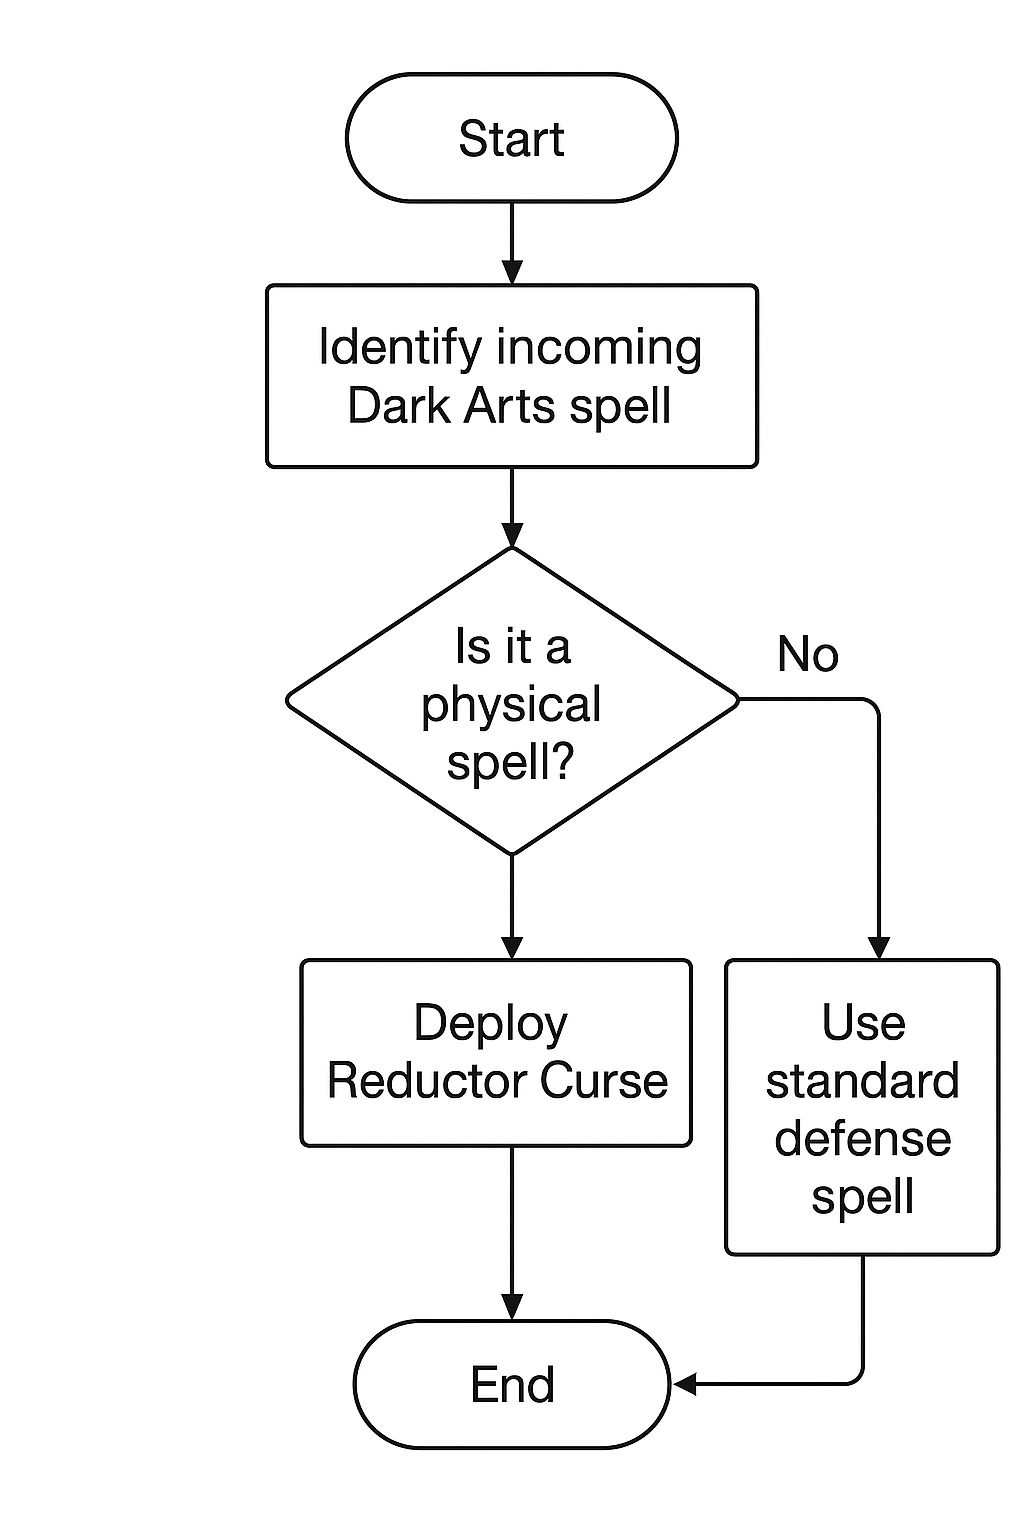
\includegraphics[width=0.5\linewidth]{images/workflow.png}
    \caption{Workflow of defensing}
    \label{fig:fig2}
\end{figure}
